% !TeX root = ../../../main.tex
\begin{figure}[htbp]
\begin{ChSixFloatBody}

\scriptsize
% \scriptsize
    % \begin{minipage}[t]{\columnwidth}
    \centering
    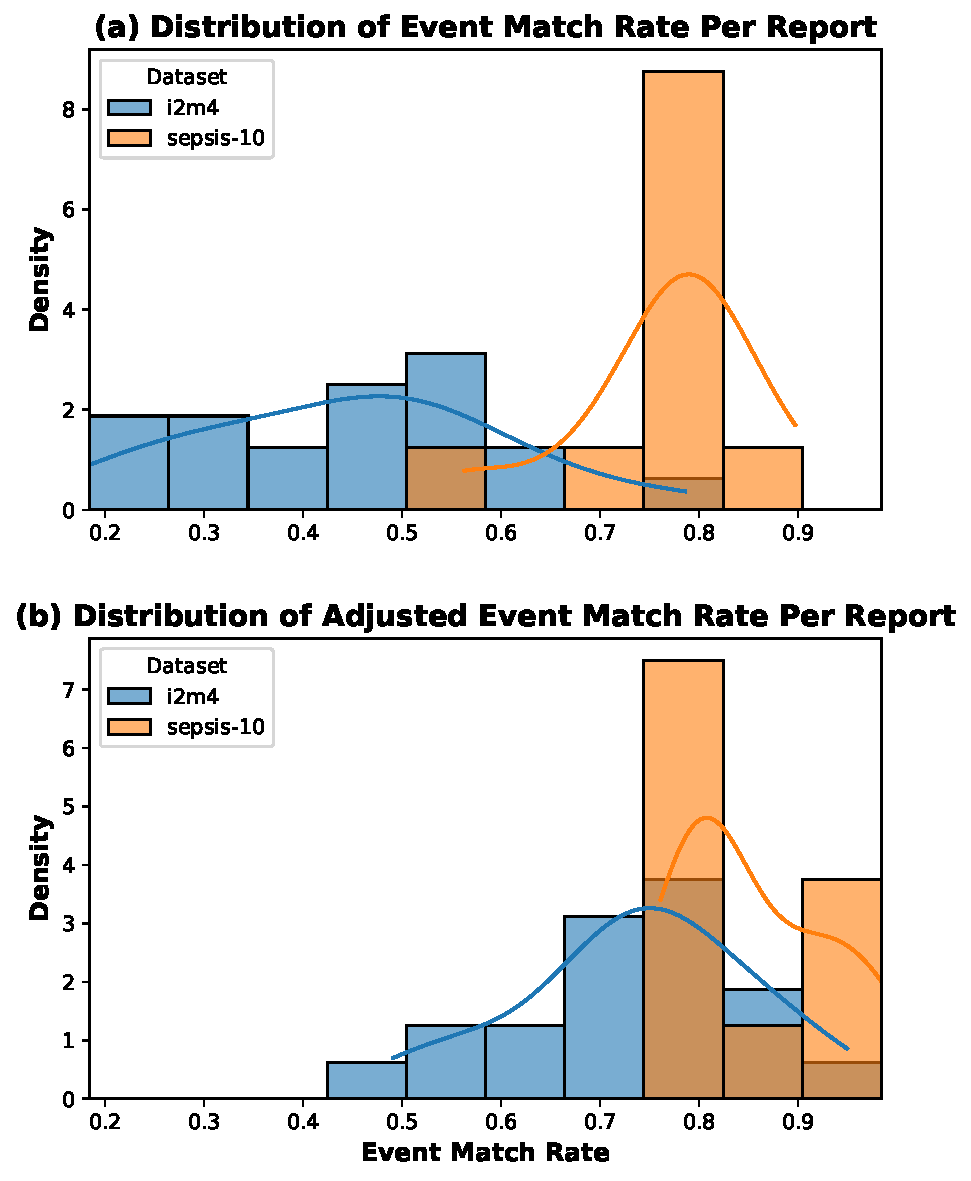
\includegraphics[width=0.7\linewidth]{Appendices/appendix-ch06/images/figures/match_rate_distributions.pdf}
    % \end{minipage}
    % \hfill
    
    

\end{ChSixFloatBody}
\caption{Distributions of Event Match Rates Across Reports Before and After Adjustment: 
    (a) Unadjusted Match Rate: Histogram and density plots of event match rates between manual annotations and Llama 3.3 predictions for reports in i2m4 (blue) and \texttt{sepsis-10} (orange). 
    The lower and more variable match rates in i2m4 highlight the impact of under-identification bias. 
    (b) Adjusted Match Rate: Histogram and density plots showing event match rates after excluding manual clinical events without Llama 3.3 counterparts. 
    The adjustment improves the match rates in i2m4, demonstrating that under-identification is the primary cause of its lower initial match rates compared to \texttt{sepsis-10}.}\ChSixFloatLabel{ch06:fig:match_rate_distributions}
\end{figure}